\documentclass[a4paper,12pt]{article}
\usepackage[papersize={8.5in,11in},left=2.64cm,right=2.64cm,top=2.64cm,bottom=2.64cm]{geometry}

\usepackage{placeins}
\usepackage{natbib}
\usepackage{lineno}
\usepackage{soul}
\usepackage{url}
\usepackage[colorlinks = true,
            linkcolor = blue,
            urlcolor  = blue,
            citecolor = blue,
            anchorcolor = blue]{hyperref}
            
\linenumbers
%\usepackage[printfigures]{figcaps}

\usepackage[colorinlistoftodos,prependcaption,textsize=tiny]{todonotes}
\usepackage{authblk}
\usepackage{setspace}
\doublespacing
\usepackage{inputenc}

\usepackage{lscape}

%\usepackage[paper=portrait,pagesize]{typearea}


\usepackage{booktabs}
\usepackage{dcolumn}

%\def\settablenum#1{\let\caption\savecaption
%\def\@captype{table}
%\def\thetable{#1} \let\@currentlabel\thetable  \let\label\savelabel}


%opening
\title{Supplementary materials for "The imbricated foreshock and aftershock activities of the Balsorano (Italy) M$_w$ 4.4 normal fault earthquake and implications for earthquake initiation"}


\author{H. S. S\'anchez-Reyes$^1$, D. Essing$^1$, E. Beauc\'e$^2$, P. Poli$^1$}

\affil[1]{Institute of Earth Sciences, University Grenoble Alpes, Grenoble \emph{38100}, France}
\affil[2]{Department of Earth, Atmospheric, and Planetary Sciences, Massachusetts Institute of Technology, Cambridge, MA, United States}
\affil[*]{Corresponding author: hugo.sanchez-reyes@univ-grenoble-alpes.fr}

\date{}                     %% if you don't need date to appear
\setcounter{Maxaffil}{0}
\renewcommand\Affilfont{\itshape\small}



\begin{document}


\maketitle

%% ------------------------------------------------------------------------ %%
%
%  TEXT
%
%% ------------------------------------------------------------------------ %%

\noindent\textbf{Contents of this file}
\begin{enumerate}
 \item Tables S1 to S4 
 \item Figures S1 to S2 
\end{enumerate}

\noindent\textbf{Additional Supporting Information}
\begin{enumerate}
  \item Seismic catalog for the seismic sequence associated to the 2019 (M$_W$ 4.4) Balsorano earthquake
\end{enumerate}




\begin{table}
\renewcommand{\thetable}{S\arabic{table}}
 \caption{General information of the 2019 M$_w$ 4.4 Balsorano earthquake. All this information is taken from the INGV's online catalog.}
 \begin{center}
 \begin{tabular}{@{}l l }
   \hline
    {\hskip 2cm Mainshock data}      &            \\
    \hline
    Magnitude				        & M$_w$ 4.4    \\
    Lat (º) / Lon (º)            	& 13.61 / 41.78  \\
    Depth (km)                      & 14.0           \\    
    NP1: \ Strike / Dip / Rake  	& 299 /	58 / -120   \\
    NP2: \ Strike / Dip / Rake     	& 166 / 42 / -51    \\
    Reported activity 			    & $\approx$ 150 events  \\
   \# Stations $<$ 100 km		    & 6         
 \end{tabular}
 \end{center}
\label{tab:general_info}
\end{table}


\begin{table}
\renewcommand{\thetable}{S\arabic{table}}
\caption{Receiver locations. The distances reported are measured with respect to the mainshock epicentral location (taken from the INGV).}
\begin{center}
 \begin{tabular}{@{} l c c c}
   \hline
    Receiver  & Lon. ($^o$) & Lat. ($^o$) & Dist. (km) \\
    \hline
 CERT & 41.94903 & 12.98176 & 72.297 \\
 GUAR & 41.79450 & 13.31229 & 33.093 \\
 INTR & 42.01154 & 13.90460 & 41.820 \\    
 POFI & 41.71743 & 13.71202 & 13.112 \\
 PTQR & 42.02193 & 13.40057 & 35.780 \\
 VVLD & 41.86965 & 13.62324 & 10.411
 \end{tabular}
\end{center}
\label{tab:general_info}
\end{table}


\begin{table}
\renewcommand{\thetable}{S\arabic{table}}
 \caption{Velocity model used for the relocation process. A V$_P$/V$_S$ ratio equal to 1.73 is assumed. Slightly modified version from the model proposed by \cite{Bagh_2007_BSC}}
 \begin{center}
 \begin{tabular}{@{} c | c}
    \hline
    Depth of top of layer (km)	& P-wave velocity (km/s)  \\
    \hline
    0.0 & 5.360 \\
    3.0 & 5.360 \\
    6.0 & 5.800 \\
    14.0 & 6.650 \\
    25.0 & 6.900 
    \end{tabular}
 \label{tab:velocitymodel}
\end{center}
\end{table}

\begin{landscape}

\begin{table}[!h]
\renewcommand{\thetable}{S\arabic{table}}
 \caption{Reference templates and phase traveltimes at the six available stations (estimated from INGV data).}
 \begin{center}
 \begin{tabular}{@{} l l c c c c c c c c c c c c}
    \hline
      & & P$_{tt}$ & P$_{tt}$ & P$_{tt}$ & P$_{tt}$ & P$_{tt}$ & P$_{tt}$ & S$_{tt}$ & S$_{tt}$ & S$_{tt}$ & S$_{tt}$ & S$_{tt}$ & S$_{tt}$   \\
      \# & Origin time     & CERT & GUAR & INTR & POFI & PTQR & VVLD & CERT & GUAR & INTR & POFI & PTQR & VVLD \\
    \hline
1 & 2019/11/07 00:37:18 & 9.63 & 5.51 & 6.9 & 3.46 & 6.37 & 3.48 & 17.09 & 9.11 & 11.95 & 5.82 & 11.28 & 5.71 \\
2 & 2019/11/07 03:21:00 & 9.72 & 5.38 & 6.92 & 3.57 & 6.62 & 3.57 & 17.15 & 9.4 & 12.12 & 5.87 & 11.36 & 5.82 \\
3 & 2019/11/07 10:37:05 & 9.69 & 5.39 & 6.93 & 3.7 & 6.52 & 3.54 & 17.15 & 9.15 & 12.05 & 6.00 & 11.38 & 5.82 \\
{4} & {2019/11/07 17:35:21} & {9.7} & {5.38} & {7.01} & {3.54} & {6.48} & {3.59} & {17.22} & {9.02} & {12.12} & {5.89} & {11.52} & {5.92} \\
5 & 2019/11/07 17:47:53 & 9.77 & 5.4 & 6.93 & 3.32 & 6.53 & 3.55 & 17.29 & 9.12 & 12.07 & 5.45 & 11.42 & 5.68 \\
6 & 2019/11/07 18:04:55 & 9.74 & 5.35 & 6.9 & 3.39 & 6.54 & 3.49 & 17.21 & 9.12 & 11.86 & 5.68 & 11.45 & 5.72 \\
7 & 2019/11/07 23:19:50 & 9.62 & 5.29 & 7.09 & 3.54 & 6.44 & 3.55 & 16.89 & 8.99 & 12.19 & 6.00 & 11.20 & 5.79 \\
8 & 2019/11/08 03:08:06 & 9.06 & 5.14 & 7.06 & 3.56 & 6.45 & 3.42 & 16.85 & 8.76 & 12.21 & 5.85 & 11.08 & 5.58 \\
9 & 2019/11/08 08:10:56 & 9.93 & 5.56 & 6.75 & 3.17 & 6.72 & 3.37 & 17.33 & 9.23 & 11.69 & 5.39 & 11.58 & 5.48 \\
10 & 2019/11/08 08:16:10 & 9.84 & 5.44 & 6.88 & 3.44 & 6.51 & 3.54 & 17.40 & 9.49 & 12.00 & 5.76 & 11.53 & 5.71 \\
11 & 2019/11/08 10:43:24 & 9.50 & 5.15 & 6.89 & 3.32 & 6.29 & 3.38 & 17.00 & 8.91 & 12.08 & 5.78 & 11.19 & 5.61 \\
12 & 2019/11/08 12:00:43 & 9.75 & 5.44 & 7.04 & 3.34 & 6.61 & 3.55 & 17.29 & 9.13 & 12.44 & 5.70 & 11.35 & 5.77 \\
13 & 2019/11/08 13:07:07 & 9.41 & 5.08 & 6.86 & 3.32 & 6.22 & 3.34 & 16.88 & 8.77 & 12.31 & 5.64 & 11.04 & 5.45 \\
14 & 2019/11/08 14:22:12 & 9.52 & 5.14 & 6.92 & 3.39 & 6.48 & 3.38 & 16.99 & 8.79 & 12.39 & 5.69 & 11.19 & 5.56 \\
15 & 2019/11/09 10:57:09 & 9.72 & 5.35 & 6.87 & 3.21 & 6.54 & 3.46 & 17.20 & 9.03 & 11.98 & 5.52 & 11.33 & 5.70 \\
16 & 2019/11/09 22:14:15 & 9.59 & 5.27 & 6.66 & 3.24 & 6.43 & 3.14 & 17.07 & 9.04 & 11.61 & 5.33 & 10.91 & 5.04 \\
17 & 2019/11/09 23:09:52 & 9.79 & 5.49 & 6.90 & 3.62 & 6.61 & 3.59 & 17.48 & 9.12 & 11.88 & 5.69 & 11.66 & 5.91 \\
18 & 2019/11/10 03:31:36 & 9.55 & 5.15 & 6.58 & 3.51 & 6.37 & 3.42 & 16.82 & 8.68 & 12.21 & 5.79 & 11.07 & 5.55 \\
19 & 2019/11/10 06:56:28 & 9.62 & 5.15 & 6.56 & 3.15 & 6.40 & 3.07 & 17.04 & 9.04 & 11.92 & 5.42 & 11.39 & 5.09 \\
20 & 2019/11/11 01:43:21 & 9.59 & 5.31 & 6.90 & 3.44 & 6.42 & 3.53 & 18.00 & 9.27 & 12.05 & 5.25 & 11.44 & 5.76 \\
21 & 2019/11/11 13:41:33 & 9.46 & 5.11 & 7.00 & 3.49 & 6.22 & 3.39 & 16.81 & 8.79 & 12.20 & 5.85 & 11.10 & 5.54 \\
22 & 2019/11/11 16:04:53 & 9.39 & 5.05 & 6.95 & 3.43 & 6.25 & 3.34 & 17.07 & 8.70 & 12.27 & 5.75 & 11.08 & 5.52 \\
23 & 2019/11/11 17:46:53 & 9.61 & 5.22 & 6.86 & 3.32 & 6.40 & 3.43 & 17.05 & 8.97 & 12.44 & 5.22 & 11.23 & 5.62
    \end{tabular}
 \label{tab:velocitymodel}
\end{center}
\end{table}

\end{landscape}


\begin{landscape}

\begin{table}
\renewcommand{\thetable}{S\arabic{table}}
 \caption{Summary of the 23 templates used for scanning the continuous data. The estimated magnitude, and relocation resulting from the analysis described in the main manuscript are compared with the information provided from the INGV. The longitude and latitude are given in geographical degrees, depth is given in kilometers and the magnitude is estimated from a linear regression (figure S3).}
 \begin{center}
 \begin{tabular}{@{} c c c c c c c c c c}
\hline
ID & Orig. time & Lon. (hh) & Lat. (hh) & Depth (hh) & Est. Mag. & INGV Lon. & INGV Lat. & INGV Depth & INGV Mag. \\
\hline 
45 & 2019-11-07 00:37:18 & 13.6061 & 41.7737 & 13.972 & 1.1734 & 13.6082 & 41.7778 & 14.2 & 1.2 \\
85 & 2019-11-07 03:21:00 & 13.6026 & 41.7744 & 13.87 & 1.3777 & 13.6117 & 41.7767 & 15.2 & 1.4 \\
153 & 2019-11-07 10:37:05 & 13.6039 & 41.7735 & 13.862 & 1.3494 & 13.6047 & 41.7775 & 15.6 & 1.3 \\
166 & 2019-11-07 17:35:21 & 13.6066 & 41.7746 & 13.94 & 4.2453 & 13.6043 & 41.7762 & 16.2 & 4.4 \\
180 & 2019-11-07 17:47:53 & 13.6054 & 41.7747 & 13.809 & 2.2965 & 13.6117 & 41.7667 & 13.4 & 2.2 \\
190 & 2019-11-07 18:04:55 & 13.6041 & 41.7739 & 14.357 & 1.4569 & 13.6128 & 41.7773 & 14.3 & 1.4 \\
274 & 2019-11-07 23:19:50 & 13.6066 & 41.7812 & 13.713 & 3.4788 & 13.5967 & 41.777 & 15.1 & 3.5 \\
357 & 2019-11-08 03:08:06 & 13.608 & 41.7778 & 14.172 & 1.4845 & 13.5908 & 41.7643 & 14.4 & 1.6 \\
423 & 2019-11-08 08:10:56 & 13.6048 & 41.7753 & 14.159 & 1.5235 & 13.6287 & 41.778 & 12.7 & 1.5 \\
425 & 2019-11-08 08:16:10 & 13.6065 & 41.7704 & 14.95 & 1.6368 & 13.6192 & 41.7772 & 14.9 & 1.6 \\
433 & 2019-11-08 10:43:24 & 13.6053 & 41.7802 & 13.877 & 2.8811 & 13.5903 & 41.78 & 12.8 & 2.6 \\
442 & 2019-11-08 12:00:43 & 13.6088 & 41.7767 & 14.029 & 1.1587 & 13.6063 & 41.766 & 14.0 & 1.1 \\
448 & 2019-11-08 13:07:07 & 13.6056 & 41.7811 & 13.719 & 1.7611 & 13.5973 & 41.7817 & 12.7 & 1.8 \\
453 & 2019-11-08 14:22:12 & 13.6035 & 41.7754 & 13.891 & 1.3305 & 13.5997 & 41.773 & 12.6 & 1.3 \\
539 & 2019-11-09 10:57:09 & 13.601 & 41.7801 & 13.947 & 1.1306 & 13.6097 & 41.7755 & 13.6 & 1.1 \\
540 & 2019-11-09 22:14:15 & 13.6147 & 41.7847 & 11.5 & 1.296 & 13.6147 & 41.7847 & 11.5 & 1.3 \\
576 & 2019-11-09 23:09:52 & 13.605 & 41.7752 & 14.298 & 1.2884 & 13.6203 & 41.7737 & 15.2 & 1.4 \\
597 & 2019-11-10 03:31:36 & 13.605 & 41.7795 & 14.343 & 1.3393 & 13.6018 & 41.7775 & 13.2 & 1.4 \\
613 & 2019-11-10 06:56:28 & 13.6069 & 41.7713 & 15.211 & 1.4618 & 13.6055 & 41.7857 & 10.8 & 1.5 \\
644 & 2019-11-11 01:43:21 & 13.6051 & 41.779 & 13.564 & 1.8014 & 13.6125 & 41.7682 & 13.5 & 1.7 \\
658 & 2019-11-11 13:41:33 & 13.6058 & 41.7765 & 13.852 & 1.6433 & 13.5912 & 41.7768 & 13.1 & 1.7 \\
665 & 2019-11-11 16:04:53 & 13.6076 & 41.779 & 13.805 & 1.5086 & 13.5938 & 41.7767 & 12.9 & 1.7 \\
674 & 2019-11-11 17:46:53 & 13.6052 & 41.772 & 12.6 & 1.2764 & 13.6052 & 41.772 & 12.6 & 1.2 \\
    \end{tabular}
 \label{tab:velocitymodel}
\end{center}
\end{table}

\end{landscape}


\begin{figure}
\renewcommand{\thefigure}{S\arabic{figure}}
\begin{center}
 \noindent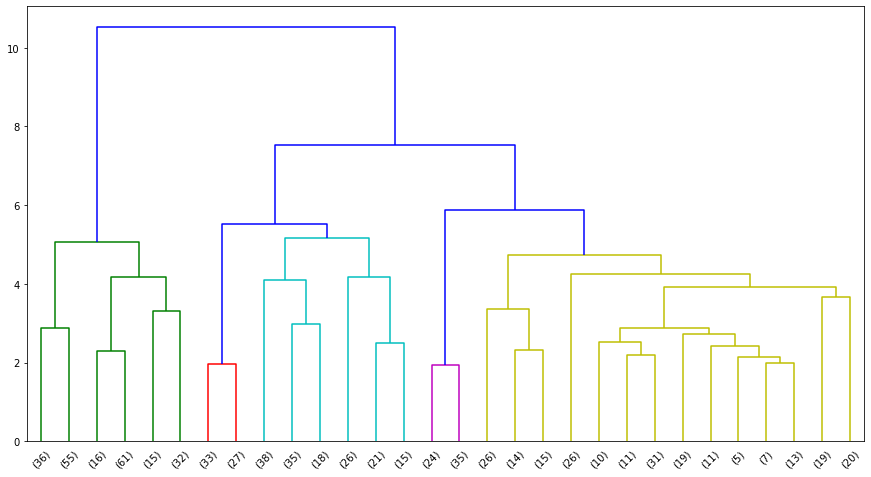
\includegraphics[width=1\linewidth]{dendrogram_balsorano.png} 
\end{center}
\caption{Dendrogram obtained from the waveform-based hierarchical clustering performed. The distance metric between two different waveforms ($i$ and $j$) is estimated as 1-C$_{ij}$. Ward's minimum variance linkage technique is used. The distance threshold to define the final number of cluster is set to 5.5 (the largest separation observed form dendrogram). The color code used for every branch represents the five different cluster identified (as in figures 3, 4 and 5 in the main manuscript).}
\label{fig:dendrogram}
\end{figure}

\begin{figure}
\renewcommand{\thefigure}{S\arabic{figure}}
\begin{center}
 \noindent 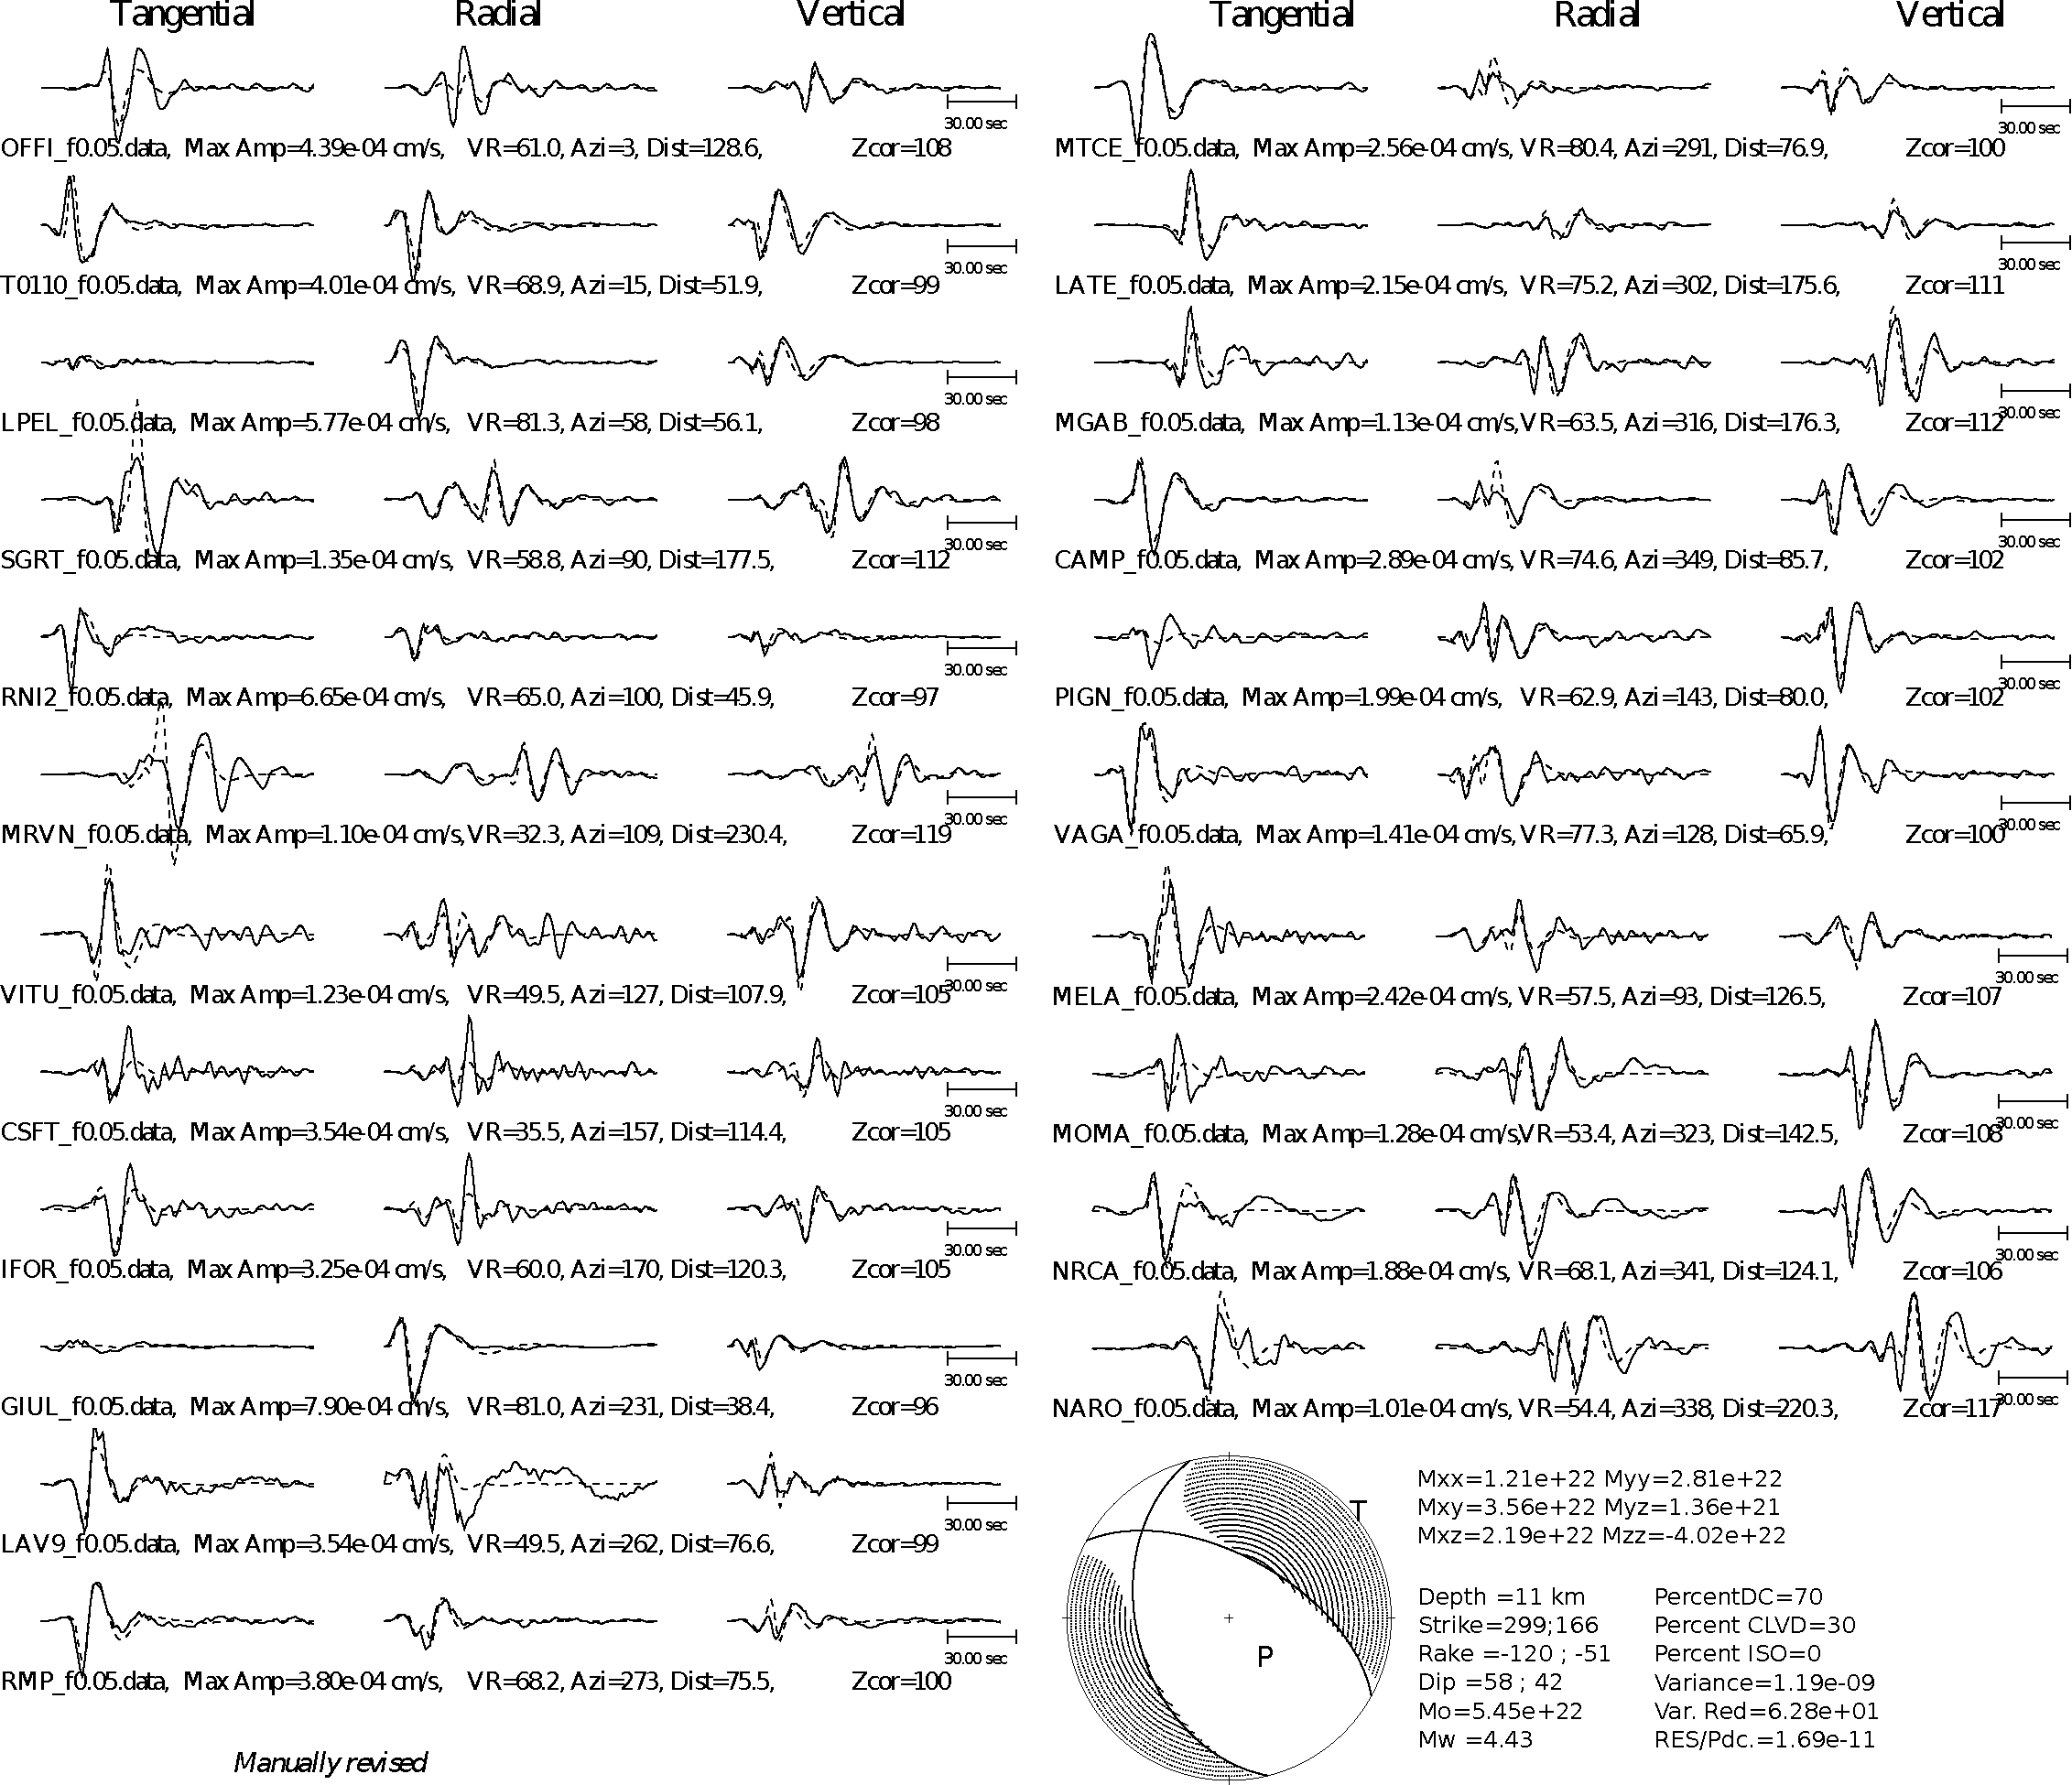
\includegraphics[width=1\linewidth]{S2_Focal_synthetics} 
\end{center}
\caption{Estimated focal mechanism and comparison of observed (solid lines) and estimated synthetic seismograms (dashed lines) for the Mw 4.4 mainshock. The three components at 22 receiver locations are shown. This figure is a modified version from the original one provided by the INGV (\url{http://webservices.ingv.it/webservices/ingv_ws_map/data/tdmt/15111/73711301_86_tdmt_reviewer_solution.pdf}).}\label{fig:S2_focal_mechanism}
\end{figure}


\begin{figure}[!h]
\renewcommand{\thefigure}{S\arabic{figure}}
\begin{center}
 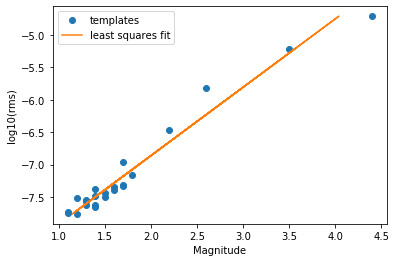
\includegraphics[width=0.8\linewidth]{S5_lsq_model.png} 
\end{center}
\caption{Least squares linear model obtained from the existing relationship between the average root mean square in the time window containing the S waves over all of the stations and components and the local magnitudes reported by the INGV for the 23 events assumed as templates. This linear model is used to estimate the magnitude of the newly detected events.}
\label{fig:S5_lsq_model}
\end{figure}


\begin{figure}[!h]
\renewcommand{\thefigure}{S\arabic{figure}}
\begin{center}
 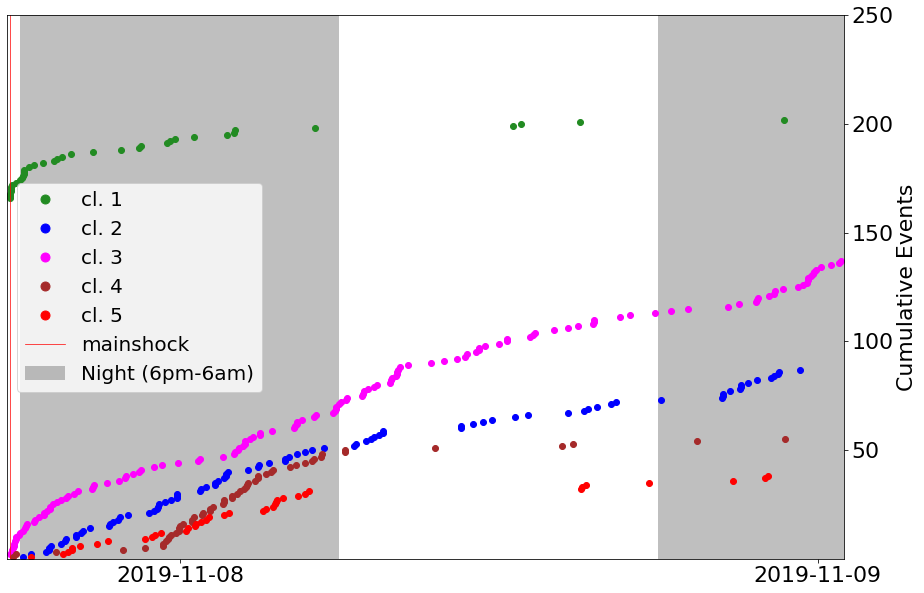
\includegraphics[width=0.8\linewidth]{S4_cumulative_per_cluster_zoom.png} 
\end{center}
\caption{Zoom in into the cumulative plot (figure 3b in the main manuscript) right after the occurrence of the mainshock.}
\label{fig:S4_fig3_zoom}
\end{figure}


\begin{figure}[!h]
\renewcommand{\thefigure}{S\arabic{figure}}
\begin{center}
 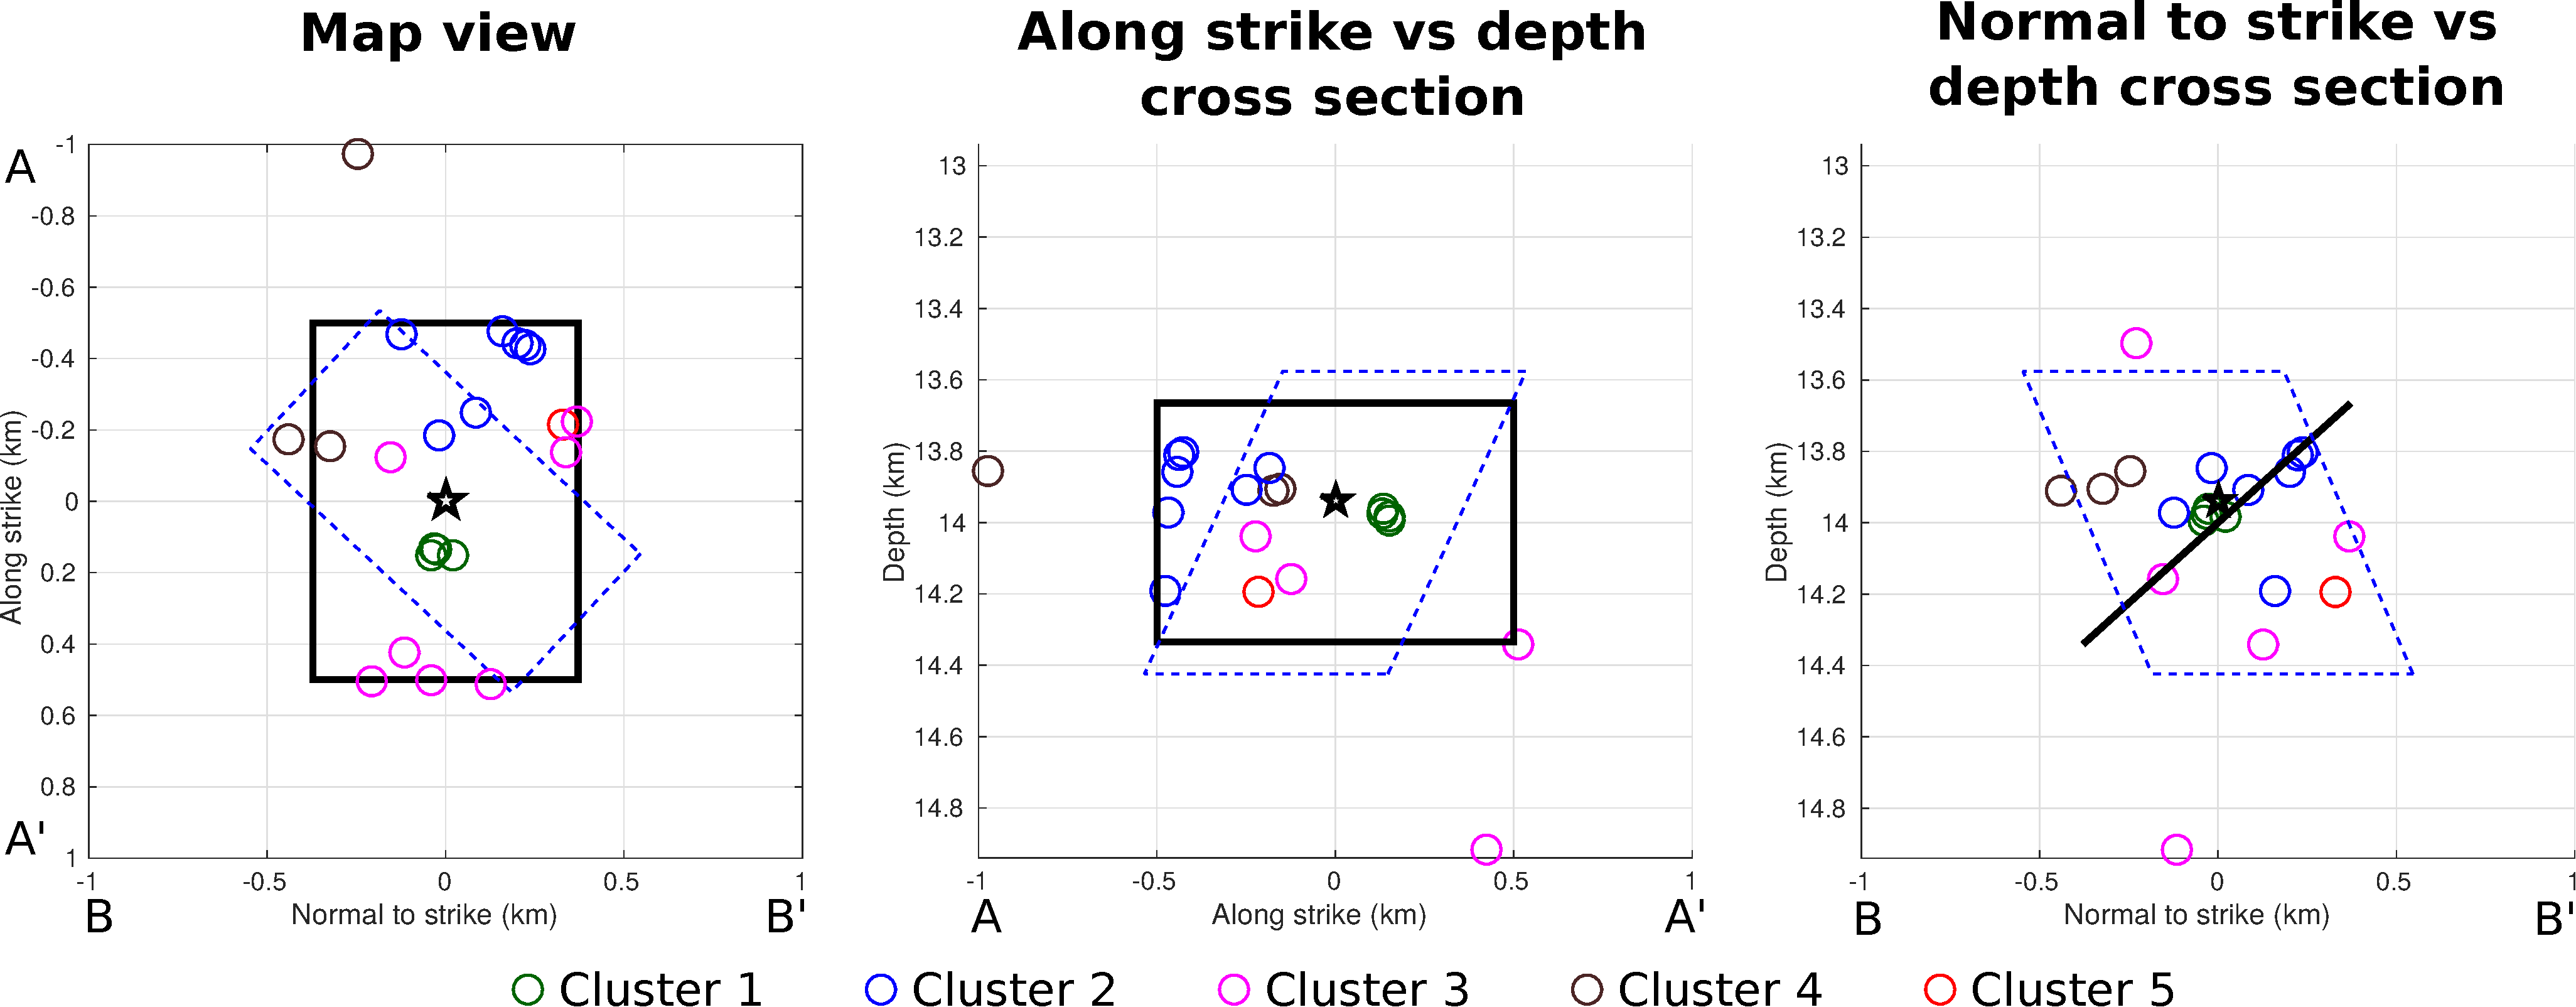
\includegraphics[width=1\linewidth]{S6_templates_per_cluster_map.pdf} 
\end{center}
\caption{Map view (left), and cross-sections along the strike (middle) and normal-strike (right) directions for the assumed main fault plane (solid black line). The dashed blue line illustrates the auxiliary plane listed in Table S1 (taken from the INGV moment tensor solution). The relative location of the 23 templates used for scanning the continuous recordings are represented by the center of the colored circles. The color code used defines to which cluster each of the templates belongs to. All of the locations are relative to the mainshock hypocenter (41.7746$^o$N 13.6066$^o$E; 13.94 km depth, black star). The directions A-A' (along strike) and B-B' (normal to the strike) are the same as in Figure 1 in the main manuscript.}
\label{fig:S6_templates_map}
\end{figure}




\FloatBarrier

\begin{thebibliography}{}

\bibitem[Bagh et~al., 2007]{Bagh_2007_BSC}
Bagh, S., Chiaraluce, L., De~Gori, P., Moretti, M., Govoni, A., Chiarabba, C.,
  Di~Bartolomeo, P., and Romanelli, M. (2007).
\newblock Background seismicity in the central apennines of italy: The abruzzo
  region case study.
\newblock {\em Tectonophysics}, 444(1-4):80--92.

\end{thebibliography}{}


\end{document}
